%!TEX root = ./template-skripsi.tex
% Gunakan \cite{citekey} untuk IEEE Style
% Gunakan \parencite{citekey} untuk APA Stle
%-------------------------------------------------------------------------------
%                            BAB II
%               TINJAUAN PUSTAKA DAN DASAR TEORI
%-------------------------------------------------------------------------------

\chapter{TINJAUAN PUSTAKA DAN DASAR TEORI}                

\section{Tinjauan Pustaka}
  Pustaka yang digunakan dalam bab ini ialah acuan primer; diutamakan artikel berkala ilmiah yang relevan dengan bidang yang diteliti, terkini, dan asli (\textit{state of the art}). Diktat dan buku ajar tidak termasuk acuan primer. Tinjauan pustaka memuat kajian singkat, jelas, dan sistematis tentang kerangka teoretis, kerangka pikir, temuan, prinsip, asumsi, dan hasil penelitian yang relevan yang melandasi masalah penelitian atau gagasan guna menggali pemahaman mengenai masalah penelitian dan pemecahan masalahnya. Oleh karena itu, dari tinjauan pustaka harus dapat diturunkan kerangka pikir, hipotesis penelitian, dan metode penelitian. Acuan yang relevan harus dimanfaatkan untuk membahas temuan yang dituangkan kemudian dalam Pembahasan. Kajian pustaka tidak sekadar berisi informasi umum seperti definisi, tetapi berisi informasi dasar yang berkaitan dengan inti penelitian. Kumpulan pustaka yang relevan dan mutakhir membantu penulis memahami perbedaan penelitiaannya dengan penelitian sebelumnya. Kumpulan pustaka yang memadai pasti akan meningkatkan kepercayaan diri penulis sewaktu memilih metode, melaksanakan penelitian, dan menyusun argumentasi dalam bab Pembahasan. Pustaka tidak boleh disitasi secara ekstensif, tetapi ditelaah dan diulas. Setiap pustaka yang diacu harus dicantumkan dalam Daftar Pustaka. Minimal memuat 5 artikel yang terpublikasikan dalam jurnal atau \textit{proceeding} \parencite{affum2021}.

\section{Landasan Teori}
  \subsection{\LaTeX}
Berisi tentang uraian, penjelasan, definisi, pengertian dasar dan ulasan yang didapat dari berbagai sumber atau referensi yang telah dipublikasikan dalam media cetak maupun elektronik (buku teks, artikel, dan lain-lain) serta terkait dengan topic skripsi. Setiap pustaka yang diacu harus dicantumkan dalam Daftar Pustaka \parencite{alden2020}.

Untuk gambar dapat dilihat di Gambar~\ref{wsn}. Pastikan gambar telah anda sebutkan didalam teks, jangan menuliskan \textbf{"Seperti terlihat pada Gambar di bawah atau di atas ini..."} namun tulislah \textbf{"Seperti terlihat pada Gambar~\ref{wsn} berikut."}.


      \begin{figure}[H]
        \centering
          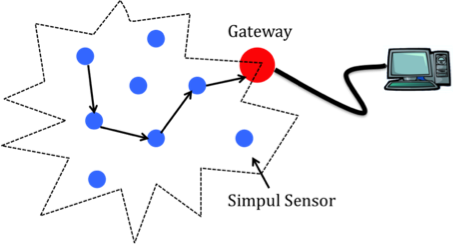
\includegraphics{gambar/wsn}
          \caption{Jaringan sensor nirkabel.}
          \label{wsn}
      \end{figure}


  \subsection{Sublime Text}
    Et affert civibus has. Has ne facer accumsan argumentum, apeirian hendrerit persequeris pro ex. Suscipit vivendum sensibus mea at, vim ei hinc numquam, at dicit timeam dissentiet mel. At patrioque intellegebat sea, error argumentum dissentias sea in.

    Quo no atqui omnesque intellegat, ne nominavi argumentum quo. Eum ei purto oporteat dissentiet, soleat utamur an sit. Et assum dicam interpretaris quo. Cetero alterum ea vel, no possit alterum utroque nec. His fuisset quaestio ad. Has eu tritani incorrupte consequuntur, esse aliquip nec ne \parencite{basconcillo2023}.
    
    
 \subsection{Aturan Penulisan}
   Ketentuan umum penulisan Laporan Skripsi:
   \begin{enumerate}[noitemsep,label=\alph*.]
   	\item   Laporan skrispsi harus dicetak (tidak boleh bolak-balik) pada kertas HVS 70 g/m2, berukuran kuarto atau A4 (21 cm x 28 cm), dan dijilid rapi dengan menggunakan sampul laminasi kertas buffalo berwarna putih.
   	\item Naskah lengkap laporan skripsi disusun dalam bahasa Indonesia yang baku, sesuai dengan ketentuan ejaan bahasa Indonesia yang disempurnakan. Apabila penulisan dalam bahasa Inggris, pedoman penulisan ejaan dan tata-bahasa mengikuti sistem spelling dan grammar berdasarkan tipe US/British English terkait dengan software yang digunakan.
   	\item Semua kalimat ditulis menggunakan tata bahasa baku. Penggunaan kata ganti orang dihindari (digunakan kalimat pasif) dan sedapat mungkin menggunakan istilah Indonesia. Apabila, karena sesuatu hal, terpaksa harus menggunakan istilah asing atau istilah daerah, istilah tersebut harus ditulis miring secara konsisten.
   	\item Dalam penulisan usulan penelitian atau tugas akhir, sebaiknya digunakan kalimat atau alinea penyambung antara definisi/teorema yang satu dengan definisi/teorema yang lain, sehingga alur isi usulan penelitian atau tugas akhir menjadi jelas. Hindari penulisan yang hanya mendaftar definisi, teorema dan lain-lainnya.
   \end{enumerate}
  
   Beberapa ketentuan tata tulis berikut perlu diperhatikan dalam penulisan usulan penelitian atau tugas akhir:
   \begin{enumerate}[noitemsep]
   	\item   Kata hubung, misalnya “maka”, “sehingga”, “sedangkan” tidak boleh digunakan sebagai awal suatu kalimat.
   	\item Penerjemahan kata “where”, “when”, dan “of” dalam bahasa Inggris tidak selalu menjadi kata “di mana”, “ketika”, dan “dari” dalam bahasa Indonesia, tetapi harus diterjemahkan/ diartikan dengan tepat, sesuai dengan bahasa Indonesia baku.
   	\item Perlu diperhatikan bahwa penulisan “ke” dan “di” sebagai awalan, harus dibedakan dengan penulisan “ke” dan “di” sebagai kata depan.
   	\item Pemenggalan kata harus dilakukan secara cermat, sesuai dengan kaidah penulisan Bahasa Indonesia yang benar.
   	\item Bilangan yang mengawali suatu kalimat harus dieja, misalnya : Sepuluh ekor tikus.
   	\item Simbol atau rumus tidak boleh berada di awal kalimat.
   	\item Tanda baca dan penulisan anak kalimat mengikuti EYD.
   \end{enumerate}
  

% Baris ini digunakan untuk membantu dalam melakukan sitasi
% Karena diapit dengan comment, maka baris ini akan diabaikan
% oleh compiler LaTeX.
\begin{comment}
\bibliography{daftar-pustaka}
\end{comment}
